\section{Mixture models}
\begin{slide}\slidetitle{Mixture models}
\tableofcontents[sectionstyle=show/hide,subsectionstyle=show/shaded/hide]

\end{slide}
%%%%%%%%%%%%%%%%%%%%%%%%%%%%%%%%%%%%%%%
\begin{slide}\slidetitle{Missing variable models}

Complexity of a model may originate from the fact
that some piece of information is {\em missing}

\vs\pause
\begin{example}
Arnason--Schwarz model with missing zones\\
Probit model with missing normal variate
\end{example}

\vs\pause
Generic representation
$$
f(\bx|\theta) = \int_\mathscr{Z} g(\bx,\bz|\theta)\,\hbox{d}\bz
$$
\end{slide}
\subsection{Mixture models}\begin{slide}
\slidetitle{Mixture models}

Models of {\it mixtures of distributions}:
$$
x \sim f_{j} \hbox{ with probability }p_{j},
$$
for $j=1, 2, \ldots, k$, with overall density
\BrickRed{$$
p_{1} f_{1}(x) +\cdots+ p_{k} f_{k}(x) \; .
$$}
\pause
Usual case: parameterised components
$$
\sum_{i=1}^k p_i f(x|\theta_i)
$$
where {\em weights} $p_i$'s are distinguished from other parameters

\end{slide}\begin{slide}\slidetitle{Motivations}

\begin{itemize}
\item  Dataset made of several latent/missing/unobserved strata/subpopulations. 
Mixture structure due to the missing origin/allocation of each observation
to a specific subpopulation/stratum. Inference on either the allocations (clustering)
or on the parameters $(\theta_i,p_i)$ or on the number of groups
\vss\pause
\item  Semiparametric perspective where mixtures are basis
approximations of unknown distributions
\end{itemize}
\end{slide}\begin{slide}\slidetitle{{\sf License}}

Dataset derived from license plate image

Grey levels concentrated on $256$ values later jittered

\vs
\centerline{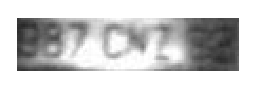
\includegraphics[width=8cm]{figures/plate.eps}}
\centerline{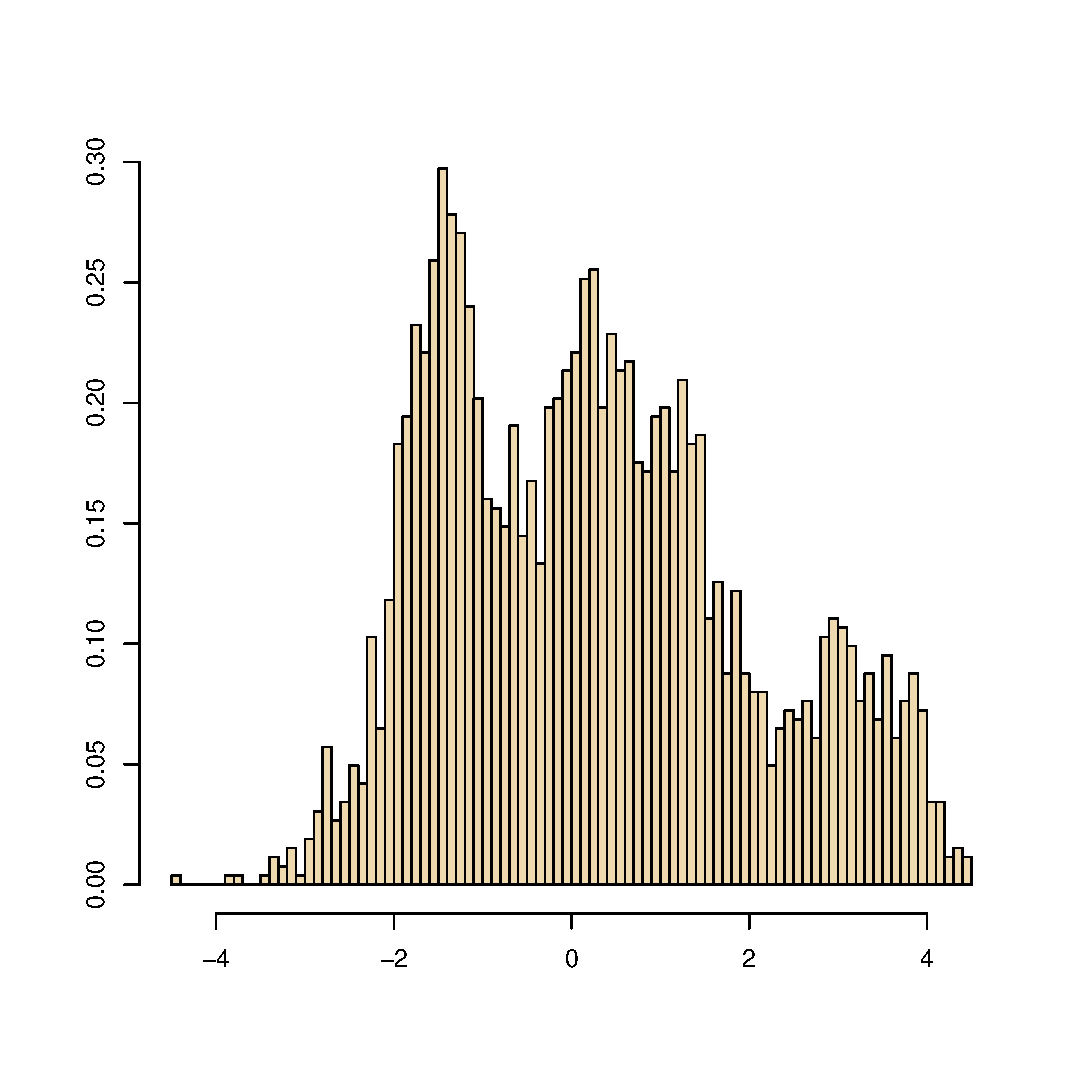
\includegraphics[height=4.5cm]{figures/plaque.hist.eps}}

\end{slide}\begin{slide}\slidetitle{Likelihood}

For a sample of independent random variables $(x_{1},\cdots,x_{n})$, likelihood
$$
\prod_{i=1}^n \left\{ p_{1} f_{1}(x_i) +\cdots+ p_{k} f_{k}(x_i) \right\} \;. 
$$

\vs\pause
Expanding this product involves 
$$
\RawSienna{k^{n}}
$$
elementary terms: prohibitive to compute in large samples.  

But likelihood still computable [pointwise] in $\text{O}(kn)$ time.
 
\end{slide}\begin{slide}\slidetitle{Normal mean benchmark}

Normal mixture
$$
p\,\mathscr{N}(\mu_1,1)+(1-p)\,\mathscr{N}(\mu_2,1)
$$
with only unknown means ($2$-D representation possible)

\begin{block}{Identifiability}
\begin{columns}\column{.45\textwidth}\small
Parameters $\mu_1$ and $\mu_2$ identifiable: $\mu_1$ cannot be confused with $\mu_2$ when
$p$ is different from $0.5$.

Presence of a spurious mode, understood by letting $p$ go to $0.5$\normalsize
\column{.5\textwidth}
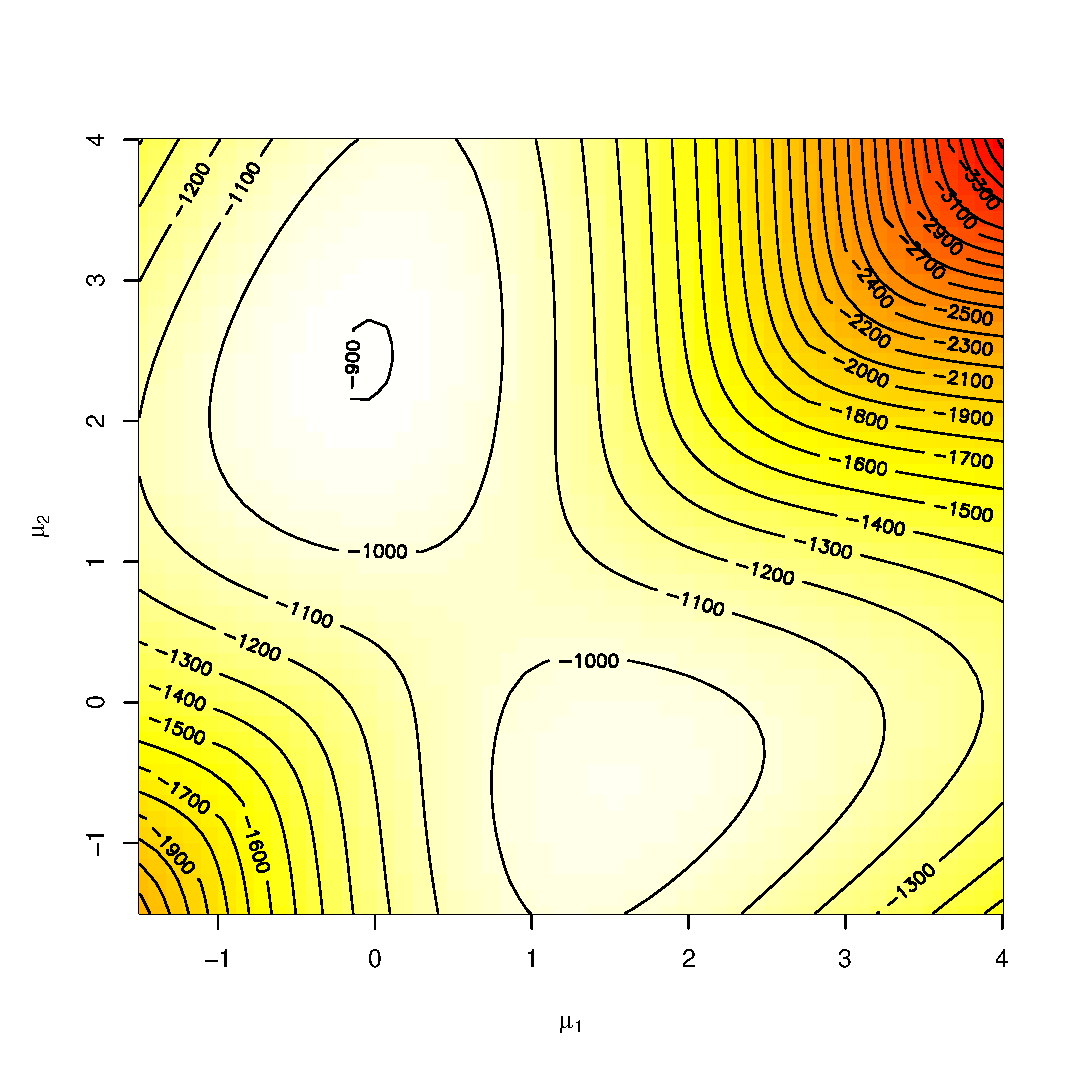
\includegraphics[width=.75\textwidth,height=.4\textheight]{figures/lvraisd1.eps}
\end{columns}
\end{block}

\end{slide}\begin{slide}
\slidetitle{Bayesian Inference}

For any prior $\pi\left(\btheta,\bp\right)$, posterior
distribution of $(\btheta,\bp)$ available up to a multiplicative constant
\small$$
\pi(\btheta,\bp|\bx) \propto \left[\prod_{i=1}^n \sum_{j=1}^k p_j\,f(x_i|\theta_j)\right] 
	\,\pi\left(\btheta,\bp\right)\,.
$$\normalsize
at a cost of order $\text{O}(kn)$

\vs\pause
\begin{block}{Difficulty}
Despite this, derivation of posterior characteristics like posterior expectations
only possible in an exponential time of order $\hbox{O}(k^n)$!
\end{block}

\end{slide}\begin{slide}
\slidetitle{Missing variable representation}

Associate to each $x_i$ a missing/latent variable $z_i$ that indicates its component:
$$
z_i|\bp\sim\mathscr{M}_k(p_1,\allowbreak\ldots,\allowbreak p_k)
$$
and
$$
x_i|z_i,\btheta \sim f(\cdot|\theta_{z_i})\,.
$$
\pause
Completed likelihood 
\small$$
\ell(\btheta,\bp|\bx,\bz)=\prod_{i=1}^n p_{z_i}\,f(x_i|\theta_{z_i})\,,
$$
and
$$
\pi(\btheta,\bp|\bx,\bz) \propto \left[\prod_{i=1}^n p_{z_i}\,f(x_i|\theta_{z_i})\right] 
\pi\left(\btheta,\bp\right)\,,
$$
\normalsize where $\bz=(z_1,\ldots,z_n)$.

\end{slide}\begin{slide}
\slidetitle{Partition sets}

Denote by $\mathcal{Z}=\{1,\ldots,k\}^n$
set of the $k^n$ possible vectors $\bz$.\\
$\mathcal{Z}$ decomposed into a partition of sets
$$
\displaystyle \mathcal{Z}=\cup_{j=1}^\mathfrak{r} \mathcal{Z}_j
$$
For a given allocation size vector
$\left(n_1,\ldots,n_k\right)$, where $n_1+\ldots+n_k=n$, 
{\em partition sets}
\small$$
\mathcal{Z}_j = \left\{\bz:\sum_{i=1}^n\mathbb{I}_{z_i=1}=n_1,
\ldots,\sum_{i=1}^n\mathbb{I}_{z_i=k}=n_k\right\}\,,
$$\normalsize
for all allocations with the given allocation size $\left(n_1,\ldots,n_k\right)$ 
and where labels $j=j(n_1,\ldots,n_k)$ defined by lexicographical ordering on the
$\left(n_1,\ldots,n_k\right)$'s.\\
%\pause\footnotesize[This means that $j=1$ corresponds to
%$\left(n_1,\ldots,n_k\right)=(n,0,\ldots,0)$, $j=2$ to
%$\left(n_1,\ldots,n_k\right)=(n-1,1,\ldots,0)$, $j=3$ to
%$\left(n_1,\ldots,n_k\right)=(n-1,0,1,\ldots,0)$, and so on.]\normalsize
%
\end{slide}\begin{slide}
\slidetitle{Posterior closed form representations}

$$
\pi\left(\btheta,\bp|\bx\right)=\sum_{i=1}^\mathfrak{r}\sum_{\bz \in\mathcal{Z}_i}
\omega\left(\bz\right) \pi\left(\btheta,\bp|\bx,\bz\right)\,,
$$
where $\omega\left(\bz\right)$ represents marginal posterior probability
of the allocation $\bz$ conditional on $\bx$
{\em [derived by integrating out the parameters $\btheta$ and $\bp$]}

\vs\pause
Bayes estimator of $\left(\btheta, \bp\right)$ 
$$
\sum_{i=1}^\mathfrak{r}\sum_{\bz\in\mathcal{Z}_i}\omega\left(\bz\right) 
\mathbb{E}^\pi\left[\btheta,\bp|\bx,\bz\right]\,.
$$

\vs\pause
\centerline{\RedOrange{\fbox{\bf \copyright\ \ Too costly: $2^n$ terms}}}

\end{slide}\subsection{MCMC approaches}
\begin{slide}
\slidetitle{General Gibbs sampling for mixture models}
Take advantage of the missing data structure:\\

\begin{block}{Algorithm}
{\sffamily
\begin{itemize}
\item  
	{\bfseries Initialization:} 
		 choose $\bp^{(0)}$ and $\btheta^{(0)}$ arbitrarily
\item  {\bfseries Step t.} For $t=1,\ldots$
\begin{enumerate}
\item Generate $z_i^{(t)}$ ($i=1,\ldots,n$) from ($j=1,\ldots,k$)
                 \begin{center}
                 $\mathbb{P}\left(z_i^{(t)}=j|p_j^{(t-1)},\theta_j^{(t-1)},x_i\right)\propto 
                 p_j^{(t-1)}f\left(x_i|\theta_j^{(t-1)}\right)$
                 \end{center}
\item Generate $\bp^{(t)}$ from $\pi(\bp|\bz^{(t)})$, 
\item Generate $\btheta^{(t)}$ from $\pi(\btheta|\bz^{(t)},\bx)$.
\end{enumerate}
\end{itemize}
}
\end{block}

\end{slide}\begin{slide}
\slidetitle{Exponential families}
When
$$
f(x|\theta)=h(x)\exp(R(\theta)\cdot T(x)>-\psi(\theta))
$$
simulation of both $\bp$ and $\btheta$
usually straightforward:\\

\RedOrange{{\bf Conjugate prior}} on $\theta_j$ given by\hyperlink{conju}{\beamerreturnbutton{Back 
to definition}}
$$
\pi_j(\theta)\propto \exp(R(\theta)\cdot \alpha_j-\beta_j\psi(\theta))\,,
$$
where $\alpha_j\in\mathbb{R}^k$ and $\beta_j>0$ are hyperparameters and
$$
\bp\sim\mathscr{D}\left(\gamma_1,\ldots,\gamma_k\right)
$$
{\em [Dirichlet distribution]}

\end{slide}\begin{slide}
\slidetitle{Gibbs sampling for exponential family mixtures}

\begin{block}{Algorithm}
{\sffamily
\begin{itemize}
\item  {\bfseries Initialization.} 
		 Choose $\bp^{(0)}$ and $\btheta^{(0)}$,
\item  {\bfseries Step t.} For $t=1,\ldots$
\begin{enumerate}
\item Generate $z_i^{(t)}$ ($i=1,\ldots,n,\,j=1,\ldots,k$) from 
         \small$$\mathbb{P}\left(z_i^{(t)}=j|p_j^{(t-1)},\theta_j^{(t-1)},x_i\right)
           \propto p_j^{(t-1)}f\left(x_i|\theta_j^{(t-1)}\right)$$ \normalsize
\item Compute $n_j^{(t)}=\sum_{i=1}^n\mathbb{I}_{z_i^{(t)}=j}$, 
		         $s_j^{(t)}=\sum_{i=1}^n\mathbb{I}_{z_i^{(t)}=j}t(x_i)$ 
\item Generate $\bp^{(t)}$ from 
	$\mathscr{D}\left(\gamma_1+n_1,\ldots,\gamma_k+n_k\right)$, 
\item Generate $\theta_j^{(t)}$ ($j=1,\dots,k$) from
  \small$$\pi(\theta_j|\bz^{(t)},\bx)\propto
  \exp\left(R(\theta_j)\cdot(\alpha+s_j^{(t)})-\psi(\theta_j)(n_j+\beta)\right).$$\normalsize
\end{enumerate}
\end{itemize}
}
\end{block}

\end{slide}\begin{slide}
\slidetitle{Normal mean example}

For mixture of two normal distributions with unknown means,
$$
p {\cal{N}}(\mu,\tau^{2}) + (1-p) {\cal{N}}(\theta,\sigma^{2}) \;,
$$
and a normal prior $\mathscr{N}\left(\delta,1/\lambda\right)$ on
$\mu_1$ and $\mu_2$, 

\end{slide}\begin{slide}
\slidetitle{Normal mean example (cont'd)}

\begin{block}{Algorithm}\small
{\sffamily
\begin{itemize}
\item  {\bfseries Initialization.} Choose $\mu_1^{(0)}$ and $\mu_2^{(0)}$,
\item  {\bfseries Step t.} For $t=1,\ldots$
\begin{enumerate}
\item Generate $z_i^{(t)}$ ($i=1,\ldots,n$) from 
                 $$\mathbb{P}\left(z_i^{(t)}=1\right)=1-\mathbb{P}\left(z_i^{(t)}=2\right)\propto
                 p\exp\left(-\frac{1}{2}\left(x_i-\mu_1^{(t-1)}\right)^2\right)$$
\item Compute $\displaystyle n_j^{(t)}=\sum_{i=1}^n\mathbb{I}_{z_i^{(t)}=j}$ and 
                 $\displaystyle (s^x_j)^{(t)}=\sum_{i=1}^n\mathbb{I}_{z_i^{(t)}=j}x_i$
\item Generate $\mu_j^{(t)}$ ($j=1,2$) from $\displaystyle 
	\mathscr{N}\left(\frac{\lambda\delta+(s^x_j)^{(t)}}{\lambda+n_j^{(t)}},
       		\frac{1}{\lambda+n_j^{(t)}}\right)$.
\end{enumerate}
\end{itemize}
}
\end{block}\normalsize

\end{slide}\begin{slide}
\slidetitle{Normal mean example (cont'd)}

\begin{columns}\column{.5\textwidth}
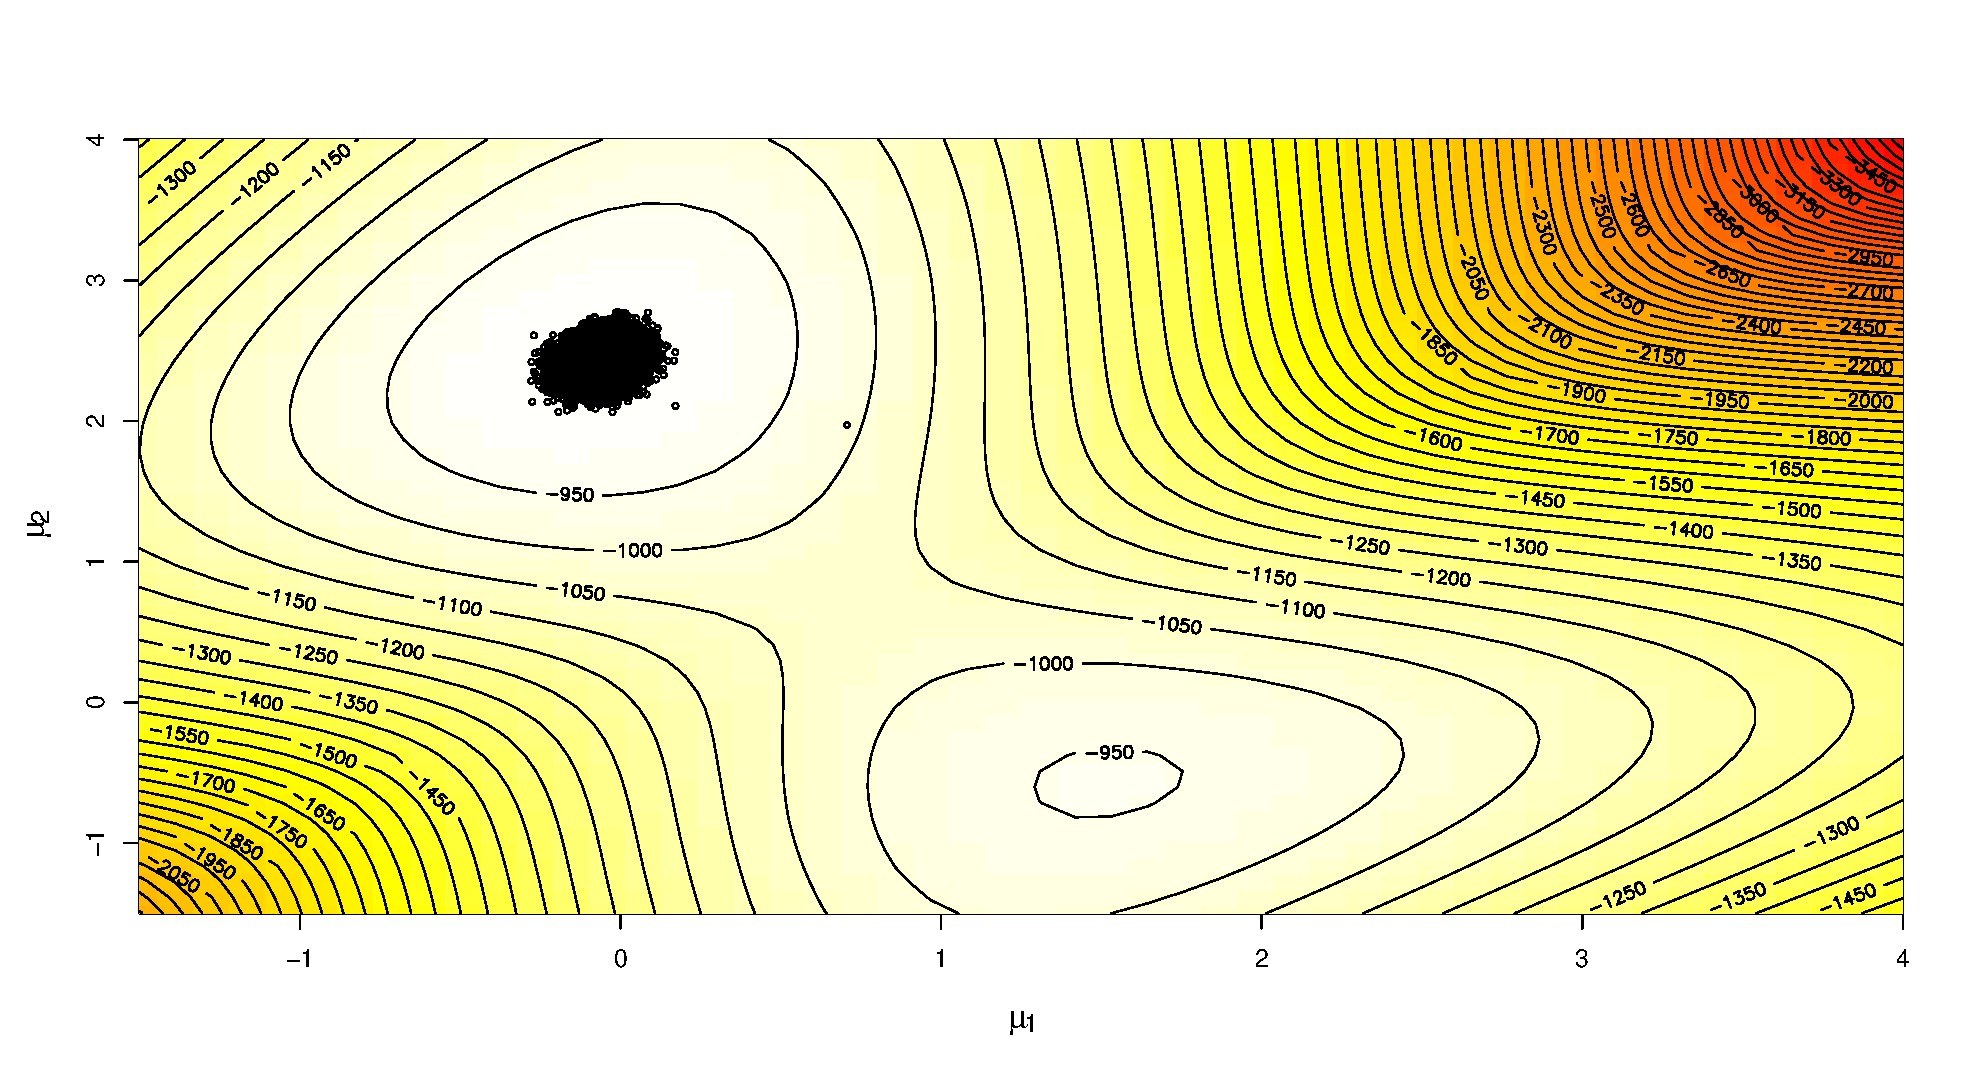
\includegraphics[width=\textwidth,height=6cm]{figures/g2n2d1.eps}\\
{\bf (a) initialised at random}
\column{.5\textwidth}
\only<2>{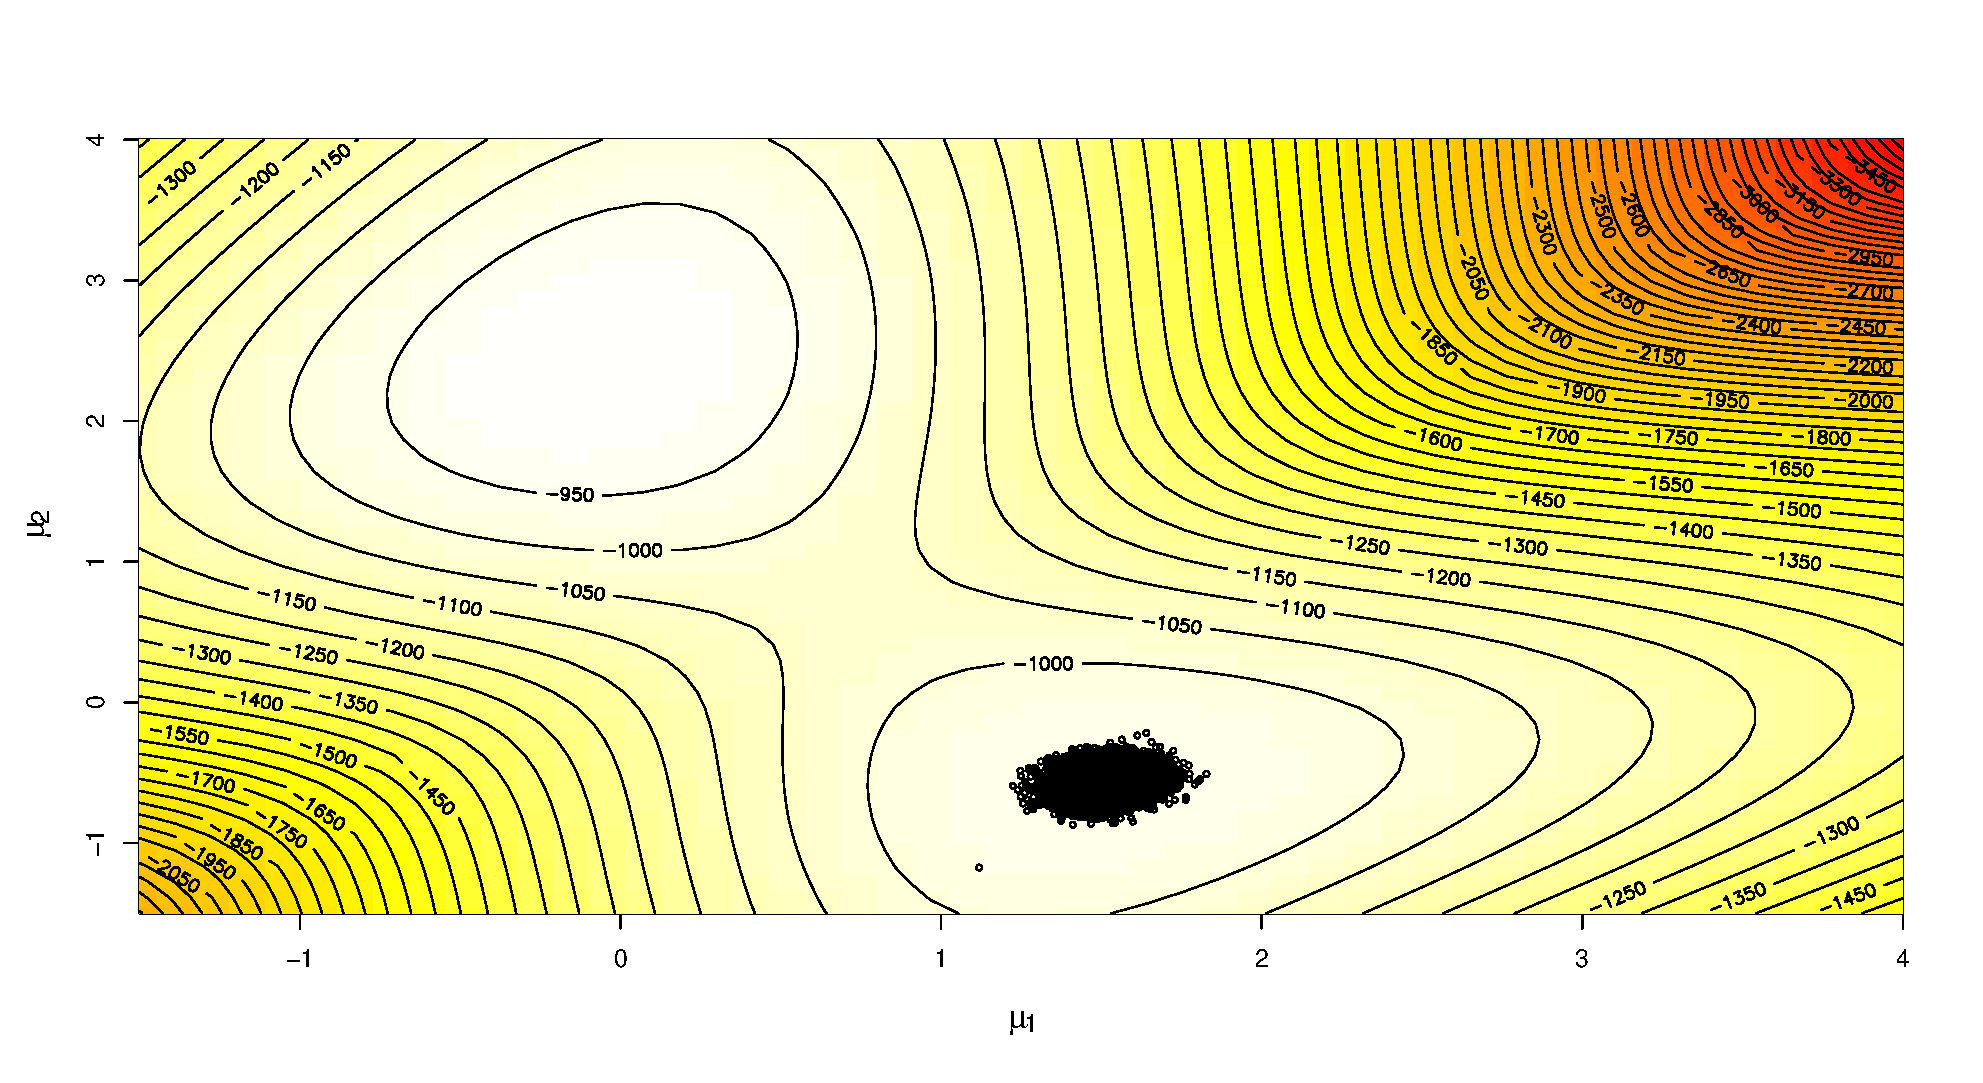
\includegraphics[width=\textwidth,height=6cm]{figures/g1n2d1.eps}\\
{\bf (b) initialised close to the lower mode}}
\end{columns}

\end{slide}\begin{slide}
\slidetitle{{\sf License}}

Consider $k=3$ components, a $\mathscr{D}_3(1/2,1/2,1/2)$ prior for the weights,
a $\mathscr{N}(\overline{x},\hat\sigma^2/3)$
prior on the means $\mu_i$ and a
$\mathscr{G}a(10,\hat\sigma^2)$ prior on the precisions
$\sigma_i^{-2}$, where $\overline{x}$ and $\hat\sigma^2$ are the
empirical mean and variance of {\sf License}
\emfarite{Empirical Bayes}

\pause
\centerline{\includegraphics[width=.8\textwidth,height=4cm]{figures/mixt.est.eps}}

\end{slide}\begin{slide}
\slidetitle{Metropolis--Hastings alternative}

For the Gibbs sampler, completion of $\bz$ increases the dimension of the simulation space 
and reduces the mobility of the parameter chain.

\vs\pause
Metropolis--Hastings algorithm available since posterior 
available in closed form, as long as $q$ provides a correct
exploration of the posterior surface, since 
$$
\frac{\pi(\btheta^\prime,\bp^\prime|\bx)}{\pi(\btheta,\bp|\bx)}\,
\frac{q(\btheta,\bp|\btheta^\prime,\bp^\prime)}{q(\btheta^\prime,\bp^\prime|\btheta,\bp)}\wedge 1
$$
computable in \BrickRed{{\bf O$(kn)$}} time

\end{slide}\begin{slide}
\slidetitle{Random walk Metropolis--Hastings}

Proposal distribution for the new value
$$
\widetilde{\theta_j}=\theta_j^{(t-1)}+u_j\hbox{ where }u_j\sim\mathscr{N}(0,\zeta^2)
$$

\vs\pause
\begin{columns}\column{.6\textwidth}
In mean mixture case, Gaussian random walk proposal is
\begin{align*}
\widetilde{\mu_1}&\sim\mathscr{N}\left(\mu_1^{(t-1)},\zeta^2\right)\quad\hbox{and}\\
\widetilde{\mu_2}&\sim\mathscr{N}\left(\mu_2^{(t-1)},\zeta^2\right)\,
\end{align*}
\column{.4\textwidth}
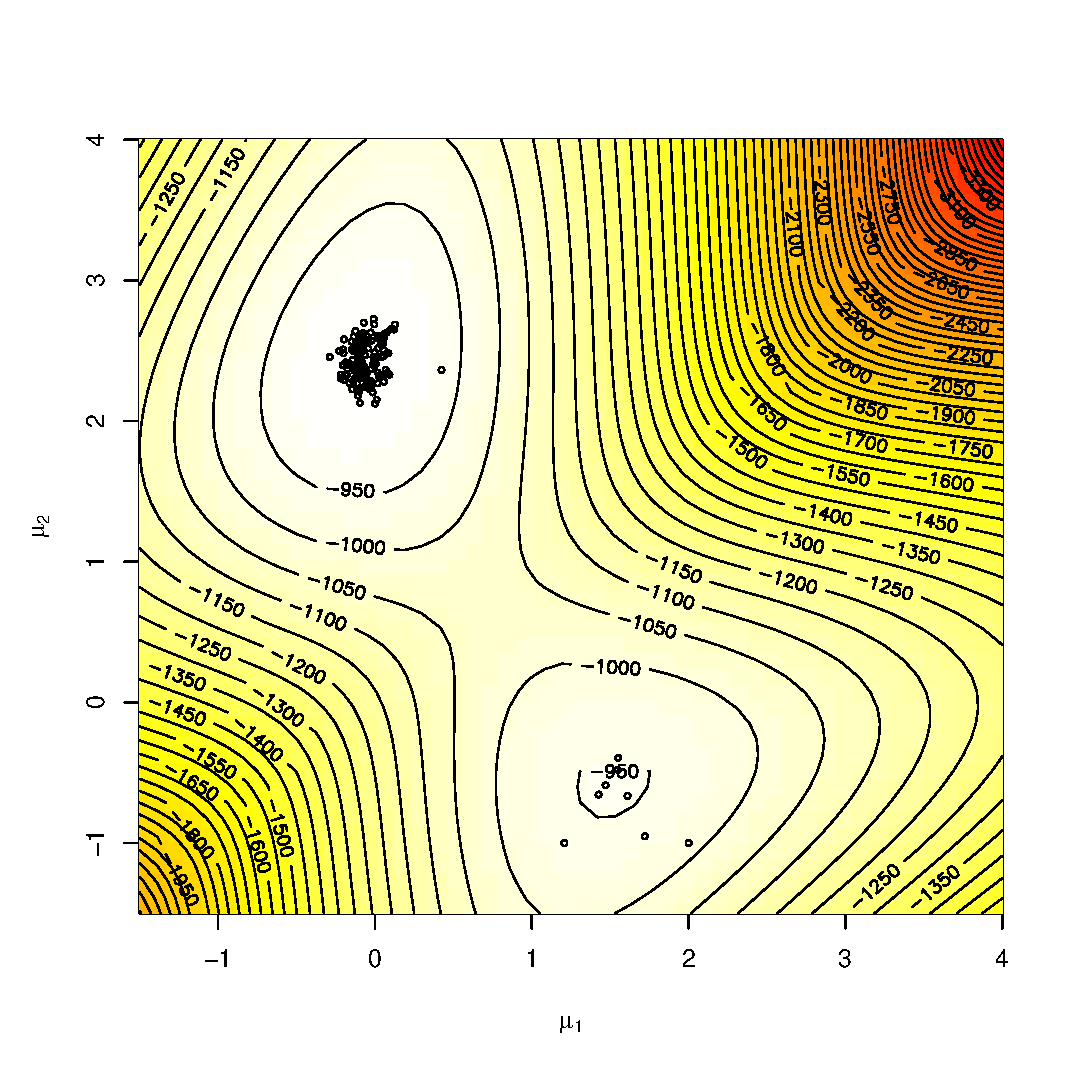
\includegraphics[height=4cm,width=4cm]{figures/hmn2d1.eps}
\end{columns}

\end{slide}\begin{slide}
\slidetitle{Random walk Metropolis--Hastings for means}

\begin{block}{Algorithm}
{\sf
\begin{itemize}
\item {\sffamily Initialization:}\\
    Choose $\mu_1^{(0)}$ and $\mu_2^{(0)}$
\item  {\sffamily Iteration $t$ $(t\ge 1)$:}
\begin{enumerate}
\item Generate $\widetilde{\mu_1}$ from $\mathscr{N}\left(\mu_1^{(t-1)},\zeta^2\right)$,
\item Generate $\widetilde{\mu_2}$ from $\mathscr{N}\left(\mu_2^{(t-1)},\zeta^2\right)$,
\item Compute
$$
r={\pi\left(\widetilde{\mu_1},\widetilde{\mu_2}|x\right)}\big/{\pi\left(\mu_1^{(t-1)},\mu_2^{(t-1)}|x\right)}
$$
\item Generate $u\sim\mathscr{U}_{[0,1]}$: if $u<r$, then 
$\left(\mu_1^{(t)}, \mu_2^{(t)}\right)=\left(\widetilde{\mu_1},\widetilde{\mu_2}\right)$ \\
                 else $\left(\mu_1^{(t)},\mu_2^{(t)}\right)=\left(\mu_1^{(t-1)},\mu_2^{(t-1)}\right)$.
\end{enumerate}
\end{itemize}
}
\end{block}

\end{slide}\begin{slide}
\slidetitle{Random walk extensions}

Difficulties with \MidnightBlue{{\bf constrained parameters}}, 
like $\bp$ such that \centerline{$\sum_{i=1}^kp_k\allowbreak=1$.}\\

\vs Resolution by overparameterisation
\small$$p_j={w_j}\bigg/{\displaystyle \sum_{l=1}^kw_l}\,,\quad w_j>0\,,$$\normalsize
and proposed move on the 
$w_j$'s 
\small$$\log(\widetilde{w_j})=\log(w_j^{(t-1)})+u_j\hbox{ where }u_j\sim\mathscr{N}(0,\zeta^2)$$
\normalsize
\vs\pause
\begin{itemize}
\item[$\lightning$] Watch out for the Jacobian in the $\log$ transform
\end{itemize}

\end{slide}\subsection{Label switching}\begin{slide}
\slidetitle{Identifiability}

A mixture model is invariant under
permutations of the indices of the components.\\

E.g., mixtures 
$$
0.3\mathscr{N}(0,1)+0.7\mathscr{N}(2.3,1)
$$
and
$$
0.7\mathscr{N}(2.3,1)+0.3\mathscr{N}(0,1)
$$
are \BurntOrange{{\bf exactly}} the same!

\vs\pause
\MidnightBlue{{\bf \copyright~ The component parameters $\theta_i$ are not identifiable {\em marginally} since
they are exchangeable}}

\end{slide}\begin{slide}
\slidetitle{Connected difficulties}

\begin{enumerate}
\item Number of modes of the likelihood of order $\mathrm{O}(k!)$:\\
\copyright~Maximization and even [MCMC] exploration of the posterior surface harder 

\pause
\item Under exchangeable priors on $(\btheta,\bp)$
{\em [prior invariant under permutation of the indices]}, all 
posterior marginals are identical:\\
\copyright~Posterior expectation of $\theta_1$ equal to posterior expectation of $\theta_2$.
\end{enumerate}

\end{slide}\begin{slide}
\slidetitle{{\sf License}}

Since Gibbs output does not produce exchangeability, the Gibbs sampler has not explored the
whole parameter space: it lacks energy to switch simultaneously enough component allocations 
at once

\centerline{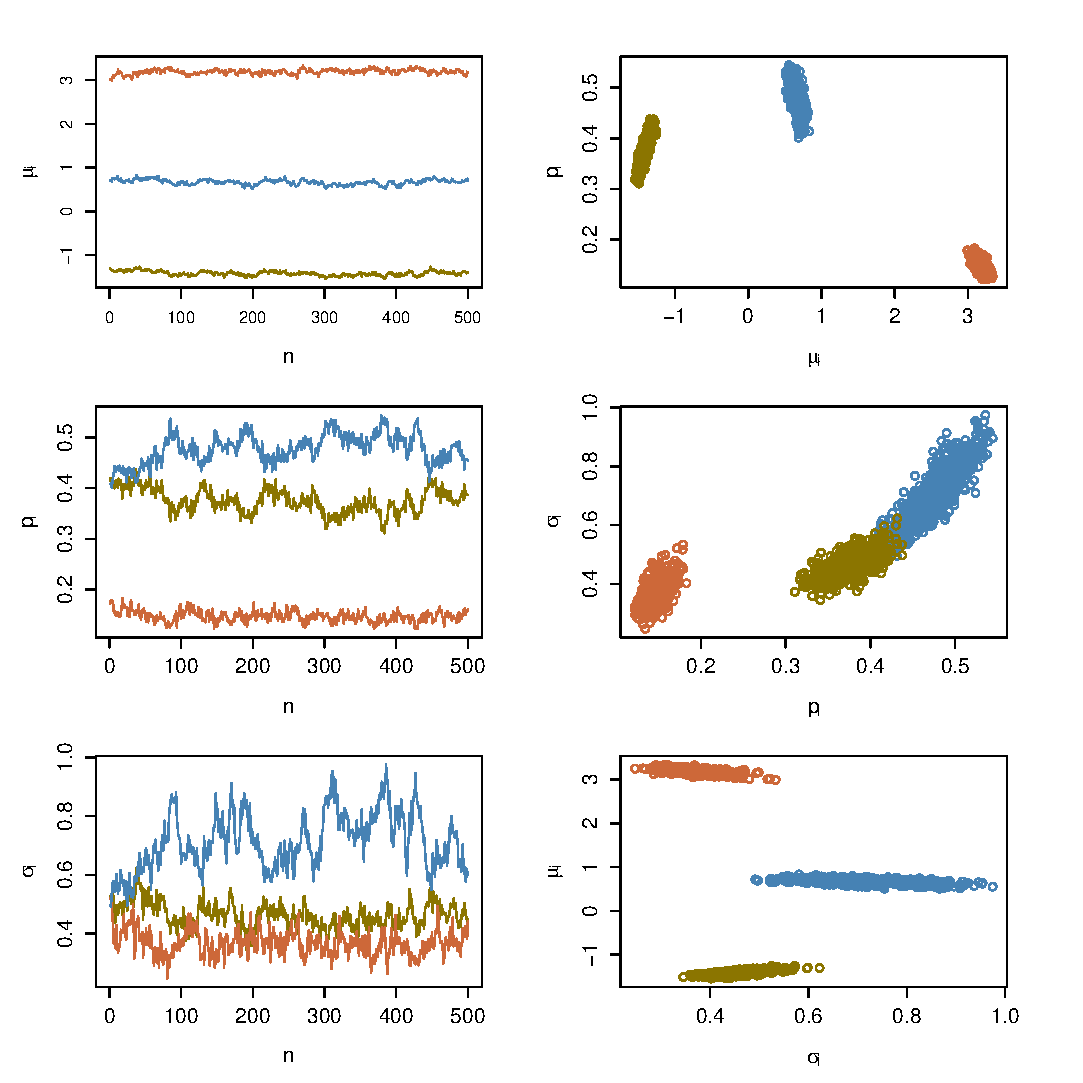
\includegraphics[height=5cm,width=10cm]{figures/mixt.noX.eps}}

\end{slide}\begin{slide}
\slidetitle{Label switching paradox}

We should observe the exchangeability of the components [label switching] to conclude
about convergence of the Gibbs sampler. 

\vs\pause If we observe it, then we do not know how to
estimate the parameters. 

\vs\pause If we do not, then we are uncertain about the convergence!!!

\end{slide}\begin{slide}
\slidetitle{Constraints}

Usual reply to lack of identifiability: impose constraints like ${\mu_1\le\ldots\le\mu_k}$
in the prior

\vs\pause Mostly incompatible with the topology of the posterior surface: posterior 
expectations then depend on the choice of the constraints.

\vs\pause
\begin{block}{Computational detail}
The constraint does not need to be imposed {\em during} the simulation
but can instead be imposed {\em after} simulation, by reordering the
MCMC output according to the constraint. This avoids possible negative effects
on convergence.
\end{block}

\end{slide}\begin{slide}
\slidetitle{Relabeling towards the mode}

Selection of one of the $k!$ modal regions of the posterior once simulation is over,
by computing the approximate MAP
\small$$
(\btheta,\bp)^{(i^*)}\quad\text{with}\quad
i^*=\arg\max_{i=1,\ldots,M} \pi\left\{ (\btheta,\bp)^{(i)}|\bx \right\}
$$\normalsize

\pause
\begin{block}{Pivotal Reordering}
At iteration $i\in\{1,\ldots,M\}$,
\begin{enumerate}
\item Compute the optimal permutation
\small$$
\tau_i=\arg\min_{\tau\in\mathfrak{S}_k} d\left(\tau\left\{
(\btheta^{(i)},\bp^{(i)}),(\btheta^{(i^*)},\bp^{(i^*)})
\right\}\right)
$$\normalsize
where $d(\cdot,\cdot)$ distance in the parameter space.
\item Set $(\btheta^{(i)},\bp^{(i)})=\tau_i((\btheta^{(i)},\bp^{(i)}))$.
\end{enumerate}
\end{block}

\end{slide}\begin{slide}
\slidetitle{Re-ban on improper priors}

Difficult to use improper priors in the setting of mixtures because independent improper priors,
$$
\pi\left(\btheta\right)=\prod_{i=1}^k\pi_i(\theta_i)\,,
\quad\text{with}\quad
\int\pi_i(\theta_i)\hbox{d}\theta_i=\infty
$$
end up, for all $n$'s, with the property
$$\int\pi(\btheta,\bp|\bx)
\hbox{d}\btheta\hbox{d}\bp=\infty\,.
$$ 

\pause
\begin{block}{Reason}
There are $(k-1)^n$ terms among the $k^n$ terms in the expansion that allocate {\em no
observation at all} to the  $i$-th component.
\end{block}

\end{slide}\begin{slide}
\slidetitle{Tempering}

Facilitate exploration of $\pi$ by flattening the target: simulate from $\pi_\alpha(x)\propto 
\pi(x)^\alpha$ for $\alpha>0$ large enough 

\vs\pause\begin{itemize}
\item Determine where the modal regions of $\pi$ are (possibly with parallel versions using
different $\alpha$'s)
\item Recycle simulations from $\pi(x)^\alpha$ into simulations from $\pi$ by importance sampling
\item Simple modification of the Metropolis--Hastings algorithm, with new acceptance
$$
\left\{ \left(\frac{\pi(\btheta^\prime,\bp^\prime|\bx)} {\pi(\btheta,\bp|\bx)}\right)^\alpha\,
\frac{q(\btheta,\bp|\btheta^\prime,\bp^\prime)} {q(\btheta^\prime,\bp^\prime|\btheta,\bp)}\right\} \wedge 1
$$
\end{itemize}

\end{slide}\begin{slide}
\slidetitle{Tempering with the mean mixture}

\includegraphics[width=11cm,height=5cm]{figures/tempix.eps}
%\includegraphics[width=4cm,height=5cm]{figures/tempix1.eps}
%\only{2-3}{\includegraphics[width=4cm,height=5cm]{figures/tempix2.eps}}
%\only<3>{\includegraphics[width=4cm,height=5cm]{figures/tempix3.eps}}

\end{slide}\subsection{MCMC for variable dimension models}\begin{slide}
\slidetitle{MCMC for variable dimension models}

\begin{columns}\column{.5\textwidth}
\small\begin{flushleft}
\begin{quote}
One of the things we do not know is\\
the number of things we do not know\\
---P.~Green, 1996---
\end{quote}
\end{flushleft}\normalsize
\column{.5\textwidth}
\begin{flushright}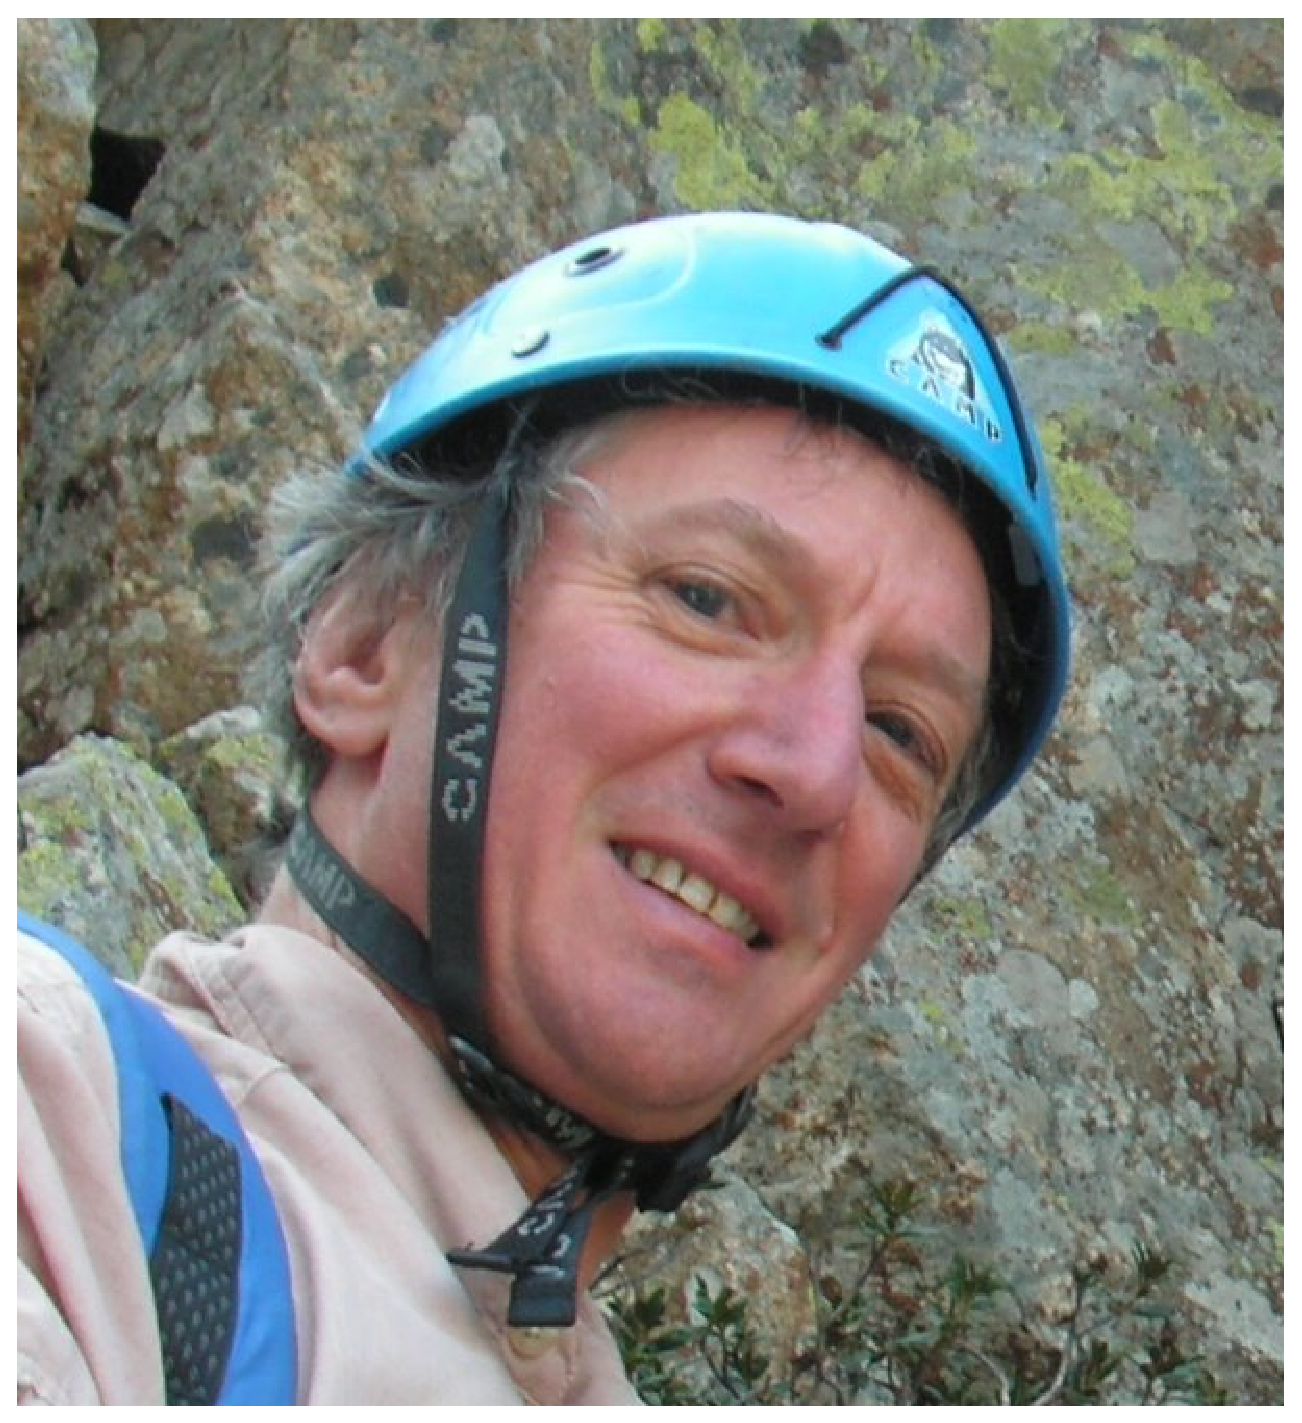
\includegraphics[width=3cm]{figures/peterG.eps}\end{flushright}
\end{columns}

\pause
\begin{example} \begin{itemize}
\item the number of components in a mixture
\item the number of covariates in a regression model
\item the number of different capture probabilities in a capture-recapture model
\item the number of lags in a time-series model
\end{itemize} \end{example}

\end{slide}\begin{slide}
\slidetitle{Variable dimension models}

Variable dimension model defined as a collection of models $(k=1.\ldots,K)$,
$$
   \GoM_k = \left\{ f(\cdot|\theta_k);\ \theta_k\in\Theta_k \right\}\,,
$$
associated with a collection of priors on the parameters of these models,
$$
  \pi_k(\theta_k)\,,
$$
and a prior distribution on the indices of these models,
$$
\left\{ \varrho(k)\,,k=1,\ldots,K \right\} \,.
$$

Global notation:
$$\RawSienna{
  \pi(\GoM_k,\theta_k) = \varrho(k)\,\pi_k(\theta_k)
}$$

\end{slide}\begin{slide}
\slidetitle{Bayesian inference for variable dimension models}

Two perspectives:
\begin{enumerate}
\item consider the variable dimension model as a {\em whole} and estimate quantities meaningful 
for the whole like predictives
\small$$
%f(x|x_1,\ldots,x_n) &= \\ &
\sum_k \hbox{Pr}({\mathfrak M}_k|x_1,\ldots,x_n)
\int \,f_k(x|\theta_k) \hbox{d}x\,\pi_k(\theta_k|x_1,\ldots,x_n) \hbox{d}\theta\,.
$$\pause\normalsize
\&\ quantities only meaningful for submodels (like moments of $\theta_k$), computed
from $\pi_k(\theta_k|x_1,\ldots,x_n)$. {\em [Usual setup]}

\item resort to testing by choosing the best submodel via
\footnotesize$$
p(\GoM_i|x) = { \displaystyle{p_i \int_{\Theta_i} f_i(x|\theta_i) 
         \pi_i(\theta_i) d\theta_i} \over
\displaystyle{\sum_j p_j \int_{\Theta_j} f_j(x|\theta_j) \pi_j(\theta_j) 
      d\theta_j}  }  
$$\normalsize
\end{enumerate}

\end{slide}\begin{slide}
\slidetitle{Green's reversible jumps}

Computational burden in exploring [possibly infinite] complex parameter space:
Green's method set up a proper measure--theoretic framework for
designing moves {\em between} models/spaces $\GoM_k$/$\Theta_k$
of varying dimensions {\em [no one-to-one correspondence]}

\vs\pause
Create a \Orange{{\bf reversible kernel}}
$\GoK$ on $\mathfrak{H}=\bigcup_k \{k\}\times\Theta_k$ such that 
$$
\int_A \int_B \GoK(x,dy) \pi(x) dx = \int_B \int_A \GoK(y,dx) \pi(y) dy
$$
for the invariant density $\pi$ [$x$ is of the form $(k,\theta^{(k)})$] 
and for all sets $A,B$ {\em [un-detailed balance]}

\end{slide}\begin{slide}
\slidetitle{Green's reversible kernel}

Since Markov kernel $\GoK$ necessarily of the form 
{\em [either stay at the same value or move to one of the states]}
$$
\GoK(x,B) = \sum_{m=1}^\infty \int \rho_m(x,y) \mathfrak{q}_m(x,dy) + \omega(x)\mathbb{I}_B(x)
$$
where $\mathfrak{q}_m(x,dy)$ transition measure to model $\GoM_m$ and $\rho_m(x,y)$
corresponding acceptance probability, \pause only need to consider proposals between two models,
$\GoM_1$ and $\GoM_2$, say.

\end{slide}\begin{slide}
\slidetitle{Green's reversibility constraint}

If transition kernels between those models are $\GoK_{1\rightarrow2}(\theta_1,d\theta)$ and
$\GoK_{2\rightarrow1}(\theta_2,d\theta)$, formal use of the \MidnightBlue{{\em detailed balance condition}
$$
\pi(d\theta_1)\, \GoK_{1\rightarrow 2}(\theta_1,d\theta) =
\pi(d\theta_2)\, \GoK_{2\rightarrow 1}(\theta_2,d\theta)\,,
$$}

\vs\pause
\begin{itemize}
\item[$\lightning$] To preserve stationarity, necessary symmetry between 
moves/proposals from $\GoM_1$ to $\GoM_2$ and from $\GoM_2$ to  $\GoM_1$
\end{itemize}


\end{slide}\begin{slide}
\slidetitle{Two-model transitions}

How to move from model $\GoM_1$ to $\GoM_2$,
with Markov chain being in state $\theta_1\in\GoM_1$ {\em [i.e. $k=1$]}?

\vs\pause
Most often $\GoM_1$ and $\GoM_2$ are of different dimensions, e.g.
\centerline{$\dim(\GoM_2)>\dim(\GoM_1)$.}

\vs In that case, need to supplement both spaces $\Theta_{k_1}$ and
$\Theta_{k_2}$ with adequate artificial spaces to create a
{\em one-to-one} mapping between them, most often by augmenting the space of
the smaller model. 

\end{slide}\begin{slide}
\slidetitle{Two-model completions}

E.g., move from  $\theta_2\in{\Theta}_2$ to ${\Theta}_1$ chosen to be
a {\em deterministic} transform of $\theta_2$
$$
\theta_1=\Psi_{2\rightarrow 1}(\theta_{2})\,,
$$

\pause
Reverse proposal expressed as
$$
\theta_2 = \Psi_{1\rightarrow 2}(\theta_1,v_{1\rightarrow 2})
$$
where $v_{1\rightarrow 2}$ r.v.~of dimension
$\dim(\GoM_2)-\dim(\GoM_1)$, generated as
$$
v_{1\rightarrow 2} \sim \varphi_{1\rightarrow 2}(v_{1\rightarrow 2})\,.
$$

\end{slide}\begin{slide}
\slidetitle{Two-model acceptance probability}

In this case, $\theta_2$ has density {\em [under stationarity]}
$$
\mathfrak{q}_{1\rightarrow 2}(\theta_2) =
\pi_1(\theta_1)\,\varphi_{1\rightarrow 2}(v_{1\rightarrow 2})\,
\left| \frac{\partial \Psi_{1\rightarrow 2}(\theta_1,v_{1\rightarrow 2})}{
             \partial (\theta_1,v_{1\rightarrow 2}) } \right|^{-1}\,,
$$
by the Jacobian rule. 

\pause
To make it $\pi_2(\theta_2)$ we thus need to accept this value with probability
$$
\alpha(\theta_1,v_{1\rightarrow 2}) = 1 \wedge \frac{\pi(\GoM_2,\theta_2)}
{\pi(\GoM_1,\theta_1)\, \varphi_{1\rightarrow 2}(v_{1\rightarrow 2})}\,
\left| \frac{\partial \Psi_{1\rightarrow 2}(\theta_1,v_{1\rightarrow 2})}{
\partial (\theta_1,v_{1\rightarrow 2}) } \right|\,.
$$

\begin{itemize}
\item[$\lightning$] This is restricted to the case when only moves between $\GoM_1$ and $\GoM_2$
		    are considered
\end{itemize}

\end{slide}\begin{slide}
\slidetitle{Interpretation}
The representation puts us back in a fixed dimension setting: 

\def\GoV{\mathfrak{V}}
\begin{itemize}
\item $\GoM_1\times\GoV_{1\rightarrow 2}$ and $\GoM_2$ in one-to-one relation.
\pause
\item reversibility imposes that $\theta_1$ is derived as
$$
(\theta_1,v_{1\rightarrow 2}) = \Psi_{1\rightarrow 2}^{-1}(\theta_2)
$$
\item appears like a {\em regular} Metropolis--Hastings move from the
couple $(\theta_1,v_{1\rightarrow 2})$ to $\theta_2$ 
when stationary distributions are
$\pi(\GoM_1,\theta_1)\times\varphi_{1\rightarrow 2}(v_{1\rightarrow 2})$
and $\pi(\GoM_2,\theta_2)$, and when proposal distribution is
{\em deterministic} (??) 
\end{itemize}

\end{slide}\begin{slide}
\slidetitle{Pseudo-deterministic reasoning}

Consider the proposals
$$
\theta_2\sim{\mathcal N}(\Psi_{1\rightarrow 2}
(\theta_1,v_{1\rightarrow 2}),\varepsilon)
\qquad\hbox{and}\qquad
\Psi_{1\rightarrow 2}(\theta_1,v_{1\rightarrow 2})\sim{\mathcal N}(\theta_2,\varepsilon)
$$

\pause Reciprocal proposal has density
\small$$
\frac{\exp\left\{-(\theta_2-\Psi_{1\rightarrow 2}
(\theta_1,v_{1\rightarrow 2}))^2/2\varepsilon\right\}}{\sqrt{2\pi\varepsilon}}
\times \left| \frac{\partial \Psi_{1\rightarrow 2}(\theta_1,v_{1\rightarrow 2})}{
     \partial (\theta_1,v_{1\rightarrow 2}) }\right|
$$\normalsize
by the Jacobian rule. 

Thus Metropolis--Hastings acceptance probability is
\small$$
1 \wedge \frac{\pi(\GoM_2,\theta_2)}{\pi(\GoM_1,\theta_1)\,
\varphi_{1\rightarrow 2}(v_{1\rightarrow 2})}\,
\left| \frac{\partial \Psi_{1\rightarrow 2}(\theta_1,v_{1\rightarrow 2})}{
\partial (\theta_1,v_{1\rightarrow 2}) }\right|
$$\normalsize

Does not depend on $\varepsilon$: \Maroon{{\bf Let $\varepsilon$ go to $0$}}

\end{slide}\begin{slide}
\slidetitle{Generic reversible jump acceptance probability}

If several models are considered simultaneously, with 
probability $\varpi_{1\rightarrow 2}$ of choosing move to $\GoM_2$ while in $\GoM_1$, 
as in 
\footnotesize$$
\GoK(x,B) = \sum_{m=1}^\infty \int \rho_m(x,y) \mathfrak{q}_m(x,dy) + \omega(x)\mathbb{I}_B(x)
$$\normalsize
\pause
acceptance probability of $\theta_2=\Psi_{1\rightarrow 2}(\theta_1,v_{1\rightarrow 2})$ is
\small$$\Red{
\alpha(\theta_1,v_{1\rightarrow 2}) =
1 \wedge \frac{\pi(\GoM_2,\theta_2)\,\varpi_{2\rightarrow 1}}
{\pi(\GoM_1,\theta_1)\,\varpi_{1\rightarrow 2}\,
\varphi_{1\rightarrow 2}(v_{1\rightarrow 2})}\,
\left| \frac{\partial \Psi_{1\rightarrow 2}(\theta_1,v_{1\rightarrow 2})}{
\partial (\theta_1,v_{1\rightarrow 2}) } \right|
}$$\normalsize
\pause while acceptance probability of $\theta_1$ with 
$(\theta_1,v_{1\rightarrow 2})=\Psi_{1\rightarrow 2}^{-1}(\theta_2)$ is
\small$$
\Red{
\alpha(\theta_1,v_{1\rightarrow 2}) =
1 \wedge \frac{\pi(\GoM_1,\theta_1)\,\varpi_{1\rightarrow 2}\,
\varphi_{1\rightarrow 2}(v_{1\rightarrow 2})}{\pi(\GoM_2,\theta_2)\,\varpi_{2\rightarrow 1}}\,
\left| \frac{\partial \Psi_{1\rightarrow 2}(\theta_1,v_{1\rightarrow 2})}{
\partial (\theta_1,v_{1\rightarrow 2}) } \right|^{-1}
}$$
\normalsize

\end{slide}\begin{slide}
\slidetitle{Green's sampler}

\begin{block}{Algorithm}
{\sffamily {\bfseries Iteration $t$ $(t\ge 1)$:} if $x^{(t)}=(m,\theta^{(m)})$,
\begin{enumerate}
\item Select model ${\mathfrak M}_n$ with probability $\pi_{mn}$
\item Generate $u_{mn}\sim\varphi_{mn}(u)$ and
                set $(\theta^{(n)},v_{nm})=\Psi_{m\rightarrow n}(\theta^{(m)},u_{mn})$
\item Take $x^{(t+1)} =( n,\theta^{(n)})$ with probability
\small$$
\min\left(
{\pi(n,\theta^{(n)}) \over \pi(m,\theta^{(m)})}
\;
{\pi_{nm} \varphi_{nm}(v_{nm}) \over \pi_{mn} \varphi_{mn}(u_{mn})}
\; \left| {\partial \Psi_{m\rightarrow n}(\theta^{(m)},u_{mn}) \over \partial
(\theta^{(m)},u_{mn})} \right|, 1 \right)
\normalsize$$
and take $x^{(t+1)} =x^{(t)}$ otherwise.
\end{enumerate}}\end{block}

\end{slide}\begin{slide}
\slidetitle{Mixture of normal distributions}
$$
\GoM_k =\left\{ (p_{jk},\mu_{jk},\sigma_{jk});\ 
\sum_{j=1}^k p_{jk} {\cal N}(\mu_{jk},\sigma_{jk}^2)\right\}
$$

\vs\pause
Restrict moves from ${\mathfrak M}_k$ to adjacent
models, like ${\mathfrak M}_{k+1}$ and ${\mathfrak
M}_{k-1}$, with probabilities $\pi_{k(k+1)}$ and $\pi_{k(k-1)}$.\\

\end{slide}\begin{slide}
\slidetitle{Mixture birth}

Take $\Psi_{k\rightarrow k+1}$ as a {\em birth step}: i.e.~add 
a new normal component in the mixture, by generating the
parameters of the new component from the prior distribution
$$
(\mu_{k+1},\sigma_{k+1})\sim \pi(\mu,\sigma)
\quad\text{and}\quad
p_{k+1}\sim\mathscr{B}e(a_1,a_2+\ldots+a_k)
$$
if $(p_1,\ldots,p_k)\sim \mathscr{M}_k(a_1,\ldots,a_k)$

\vs
Jacobian is $(1-p_{k+1})^{k-1}$

\vs\pause {\em Death step} then 
derived from the reversibility constraint by removing 
one of the $k$ components at random.

\end{slide}\begin{slide}
\slidetitle{Mixture acceptance probability}

Birth acceptance probability 
\begin{align}
&\min\left( \frac{ \pi_{(k+1)k}}{\pi_{k(k+1)} }\,\frac{(k+1)!}{(k+1)k!}
\frac{\pi({k+1},\theta_{k+1})}{\pi({k},\theta_{k})\,(k+1)\varphi_{k(k+1)}(u_{k(k+1)})}\,
,1 \right)\nonumber\\
&\quad = \min\left( \frac{ \pi_{(k+1)k}}{\pi_{k(k+1)} }\,
\frac{\varrho(k+1)}{\varrho(k)}\,
\frac{\ell_{k+1}(\theta_{k+1})\,(1-p_{k+1})^{k-1}}{\ell_{k}(\theta_{k})}
,1 \right)\,,\nonumber
\end{align}
where $\ell_k$ likelihood of the $k$ component mixture model
${\mathfrak M}_k$ and $\varrho(k)$ prior probability of model
${\mathfrak M}_k$. 

\pause \small Combinatorial terms:  there are $(k+1)!$ ways of defining a
$(k+1)$ component mixture by adding one component, while, given a $(k+1)$ component mixture,
there are $(k+1)$ choices for a component to die and then $k!$ associated mixtures for the
remaining components.\normalsize

\end{slide}\begin{slide}
\slidetitle{{\sf License}}

\only<1>{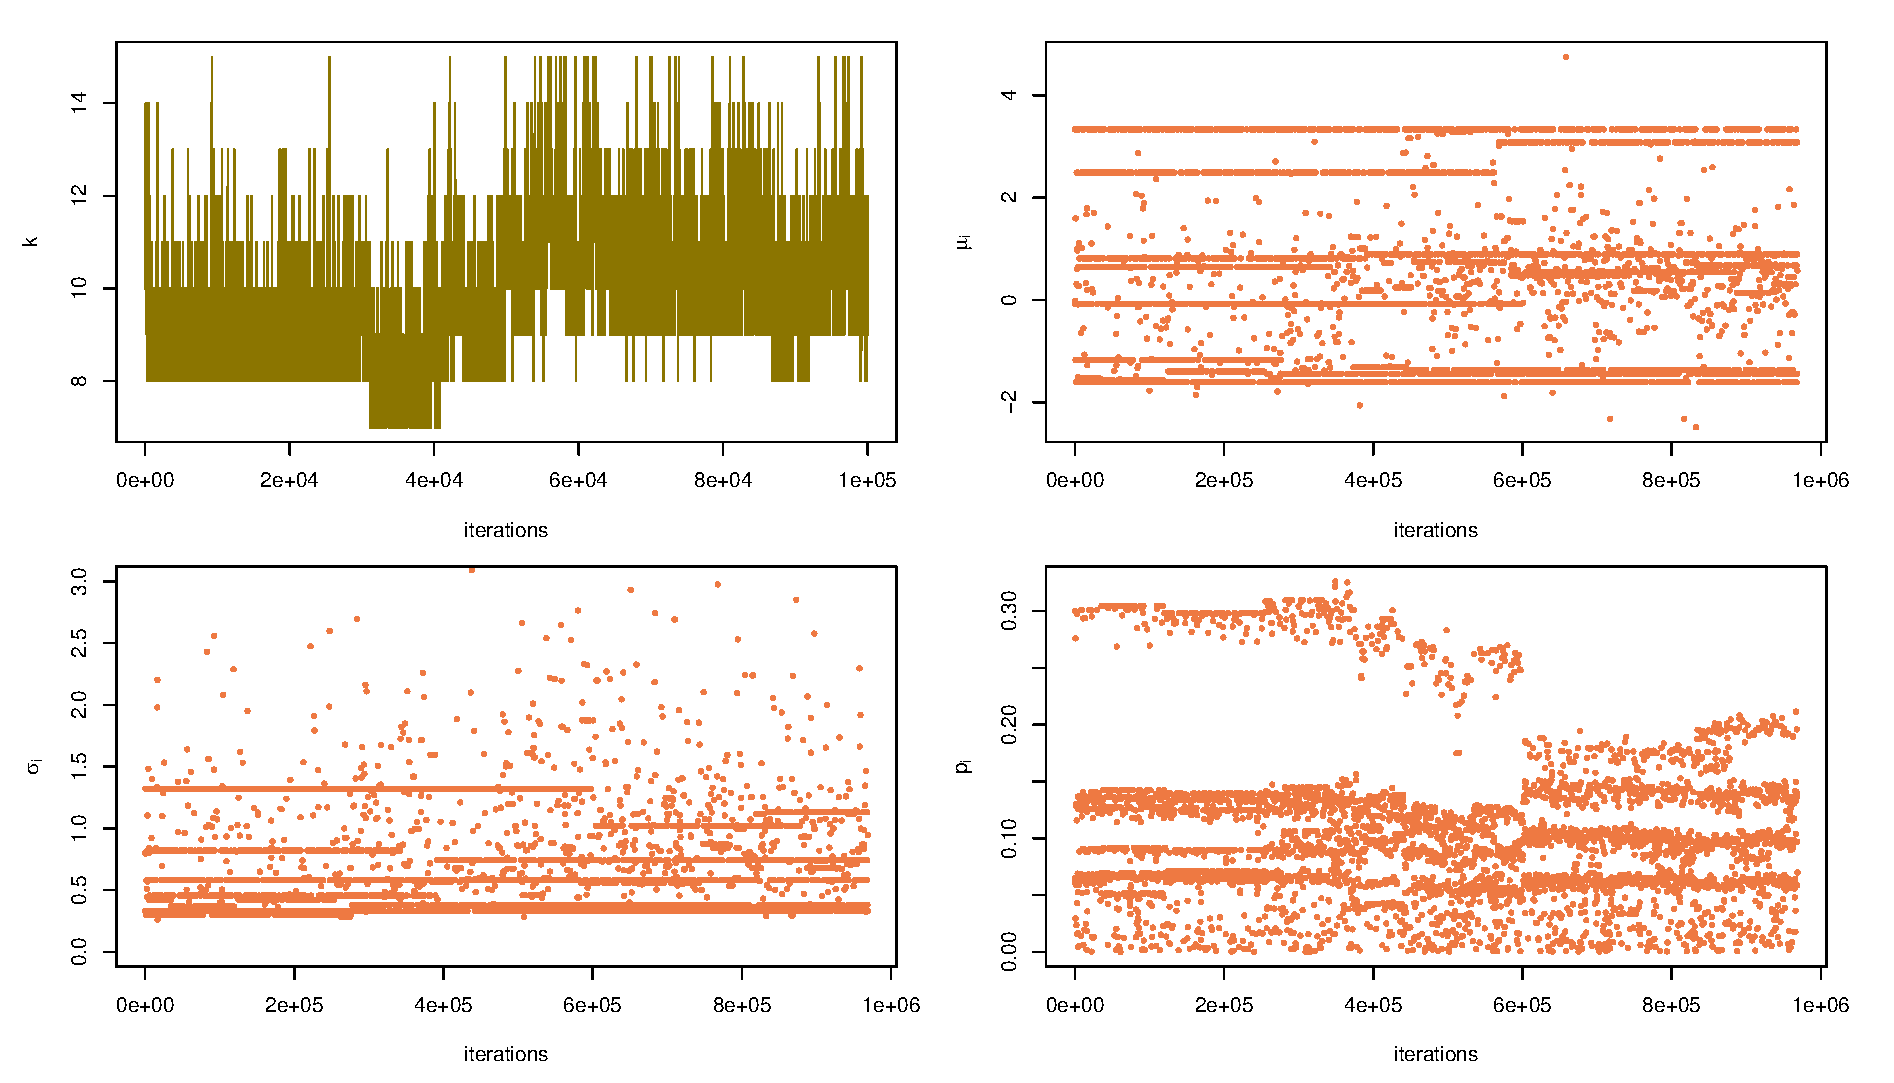
\includegraphics[width=11cm,height=7cm]{figures/mixt.rj.eps}}
\only<2>{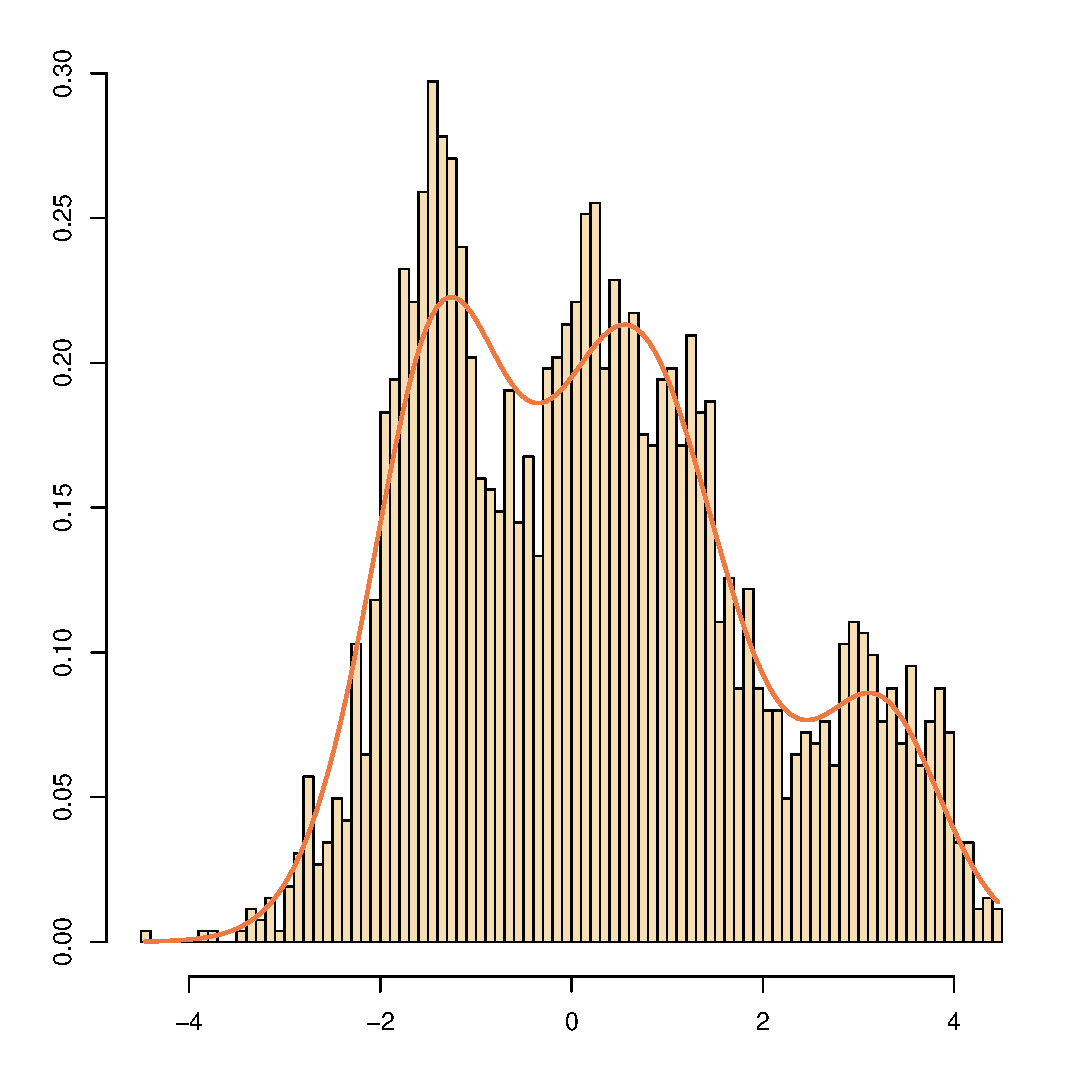
\includegraphics[width=12cm,height=7cm]{figures/mixt.rj.est.eps}}

\end{slide}\begin{slide}
\slidetitle{More coordinated moves}

Use of local moves that preserve structure of the original model.

\vs {\em Split} move from
${\mathfrak M}_k$ to ${\mathfrak M}_{k+1}$: replaces a random component, say
the $j$th, with two new components, say the $j$th and the $(j+1)$th,
that are {\em centered} at the earlier $j$th component.  And opposite {\em merge} move
obtained by joining two components together.

\end{slide}\begin{slide}
\slidetitle{Splitting with moment preservation}

Split parameters for instance created under a \MidnightBlue{{\em moment preservation
condition:}}
\small$$
\begin{array}{lll}
p_{jk} &=& p_{j(k+1)} +  p_{(j+1)(k+1)} \,, \\
p_{jk} \mu_{jk} &=& p_{j(k+1)} \mu_{j(k+1)} + p_{(j+1)(k+1)}
          \mu_{(j+1)(k+1)}\,,\\
p_{jk} \sigma_{jk}^2 &=& p_{j(k+1)} \sigma_{j(k+1)}^2 + p_{(j+1)(k+1)}
    \sigma_{(j+1)(k+1)}^2\,.
\end{array}
$$\normalsize

\pause
\begin{columns}\column{.4\textwidth}
Opposite {\em merge} move obtained by reversibility constraint
\column{.6\textwidth}
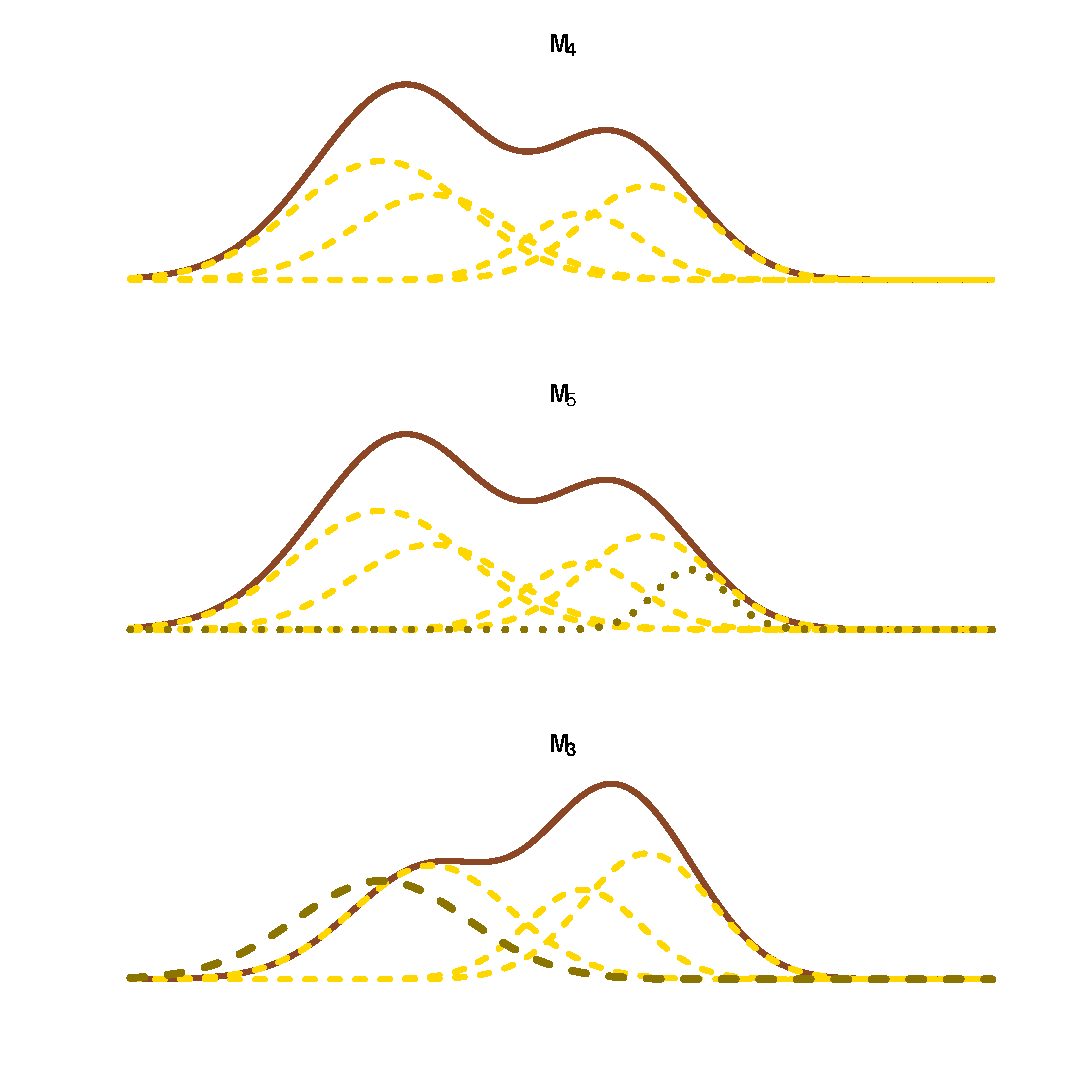
\includegraphics[width=5cm,height=4cm]{figures/birthandeath.eps}
\end{columns}

\end{slide}\begin{slide}
\slidetitle{Splitting details}

Generate the auxiliary variable $u_{k(k+1)}$ as 
$$
u_1,u_3\sim{\mathcal U}(0,1), u_2\sim\mathscr{N}(0,\tau^2)
$$
and take
$$
\begin{array}{rclrcl}
p_{j(k+1)}        &=&  u_1 p_{jk}\,,  &\quad
p_{(j+1)(k+1)} &=&  (1-u_1)p_{jk}\,,  \\
\mu_{j(k+1)}      &=&  \mu_{jk}+u_2 \,,&\quad
\mu_{(j+1)(k+1)}  &=&  \mu_{jk}-\frac{p_{j(k+1)}u_2}{p_{jk}-p_{j)(k+1)}}\,,\\
\sigma_{j(k+1)}^2 &=&  u_3 \sigma_{jk}^2\,, &\quad
\sigma_{(j+1)(k+1)} &=& \frac{p_{jk}-p_{j(k+1)}u_3}{p_{jk}-p_{j(k+1)}}\sigma_{jk}^2
\,.
\end{array}
$$

\end{slide}\begin{slide}
\slidetitle{Jacobian}

Corresponding Jacobian
\footnotesize
$$
\text{det}\left(\begin{matrix}
u_1 &1-u_1 &\cdots &\cdots &\cdots &\cdots \\
p_{jk} &-p_{jk} &\cdots &\cdots &\cdots &\cdots \\
0 &0 &1 &1 &\cdots &\cdots \\
0 &0 &1 &\frac{-p_{j(k+1)}}{p_{jk}-p_{j(k+1)}} &\cdots &\cdots \\
0 &0 &0 &0 &u_3 &\frac{p_{jk}-p_{j(k+1)}u_3}{p_{jk}-p_{j(k+1)}}\\
0 &0 &0 &0 &\sigma_{jk}^2\ &\frac{-p_{j(k+1)}}{p_{jk}-p_{j(k+1)}}\sigma_{jk}^2\\
\end{matrix}\right)
= \frac{p_{jk}}{(1-u_1)^2}\,\sigma_{jk}^2
$$\normalsize

\end{slide}\begin{slide}
\slidetitle{Acceptance probability}

Corresponding split acceptance probability
\small$$
\min\left(\frac{\widetilde\pi_{(k+1)k}}{\widetilde\pi_{k(k+1)} }\,\frac{\varrho(k+1)}{\varrho(k)}\,
\frac{\pi_{k+1}(\theta_{k+1})\ell_{k+1}(\theta_{k+1})}{\pi_{k}(\theta_{k})\ell_{k}
(\theta_{k})}\,\frac{p_{jk}}{(1-u_1)^2}\,\sigma_{jk}^2,1 \right)
$$\normalsize
where $\widetilde\pi_{(k+1)k}$ and $\widetilde\pi_{k(k+1)}$ denote split and merge probabilities
when in models $\mathfrak{M}_k$ and $\mathfrak{M}_{k+1}$

\vs\pause\small
Factorial terms vanish: for a split move there are $k$ possible choices
of the split component and then $(k+1)!$ possible orderings of the $\theta_{k+1}$ vector \pause
while, for a merge, there are $(k+1)k$ possible choices for the components to be merged
and then $k!$ ways of ordering the resulting $\theta_k$.\normalsize

\end{slide}
